\begin{chapter}{Kapitel}
 \section*{Chapter 1.1}
 \f{Definition Eingebettetes System:}
 \vspace*{3pt}
 
 \noindent \ku{Ein eingebettetes System ist ein informationsverarbeitendes System bestehend aus Hardware und Software, das in einem technischen Gesamtsystem eingebettet 
 ist, dessen primärer Zweck nicht das Verarbeiten und Aufbereiten von Information ist.}\\
 \vspace*{5pt}
 
 \noindent Durch die zunehmende Komplexität hat sich der Entwurf eingebetteter Systeme von analogen Schaltungen und Assemblerprogrammen auf einfachen 
 Mikrokontrollern weg zum Problem hin entwickelt, komplexe Hardware/Software Systeme mittels leistungsfähiger Werkzeuge zu entwickeln und zu optimieren.
 \vspace*{5pt}
 
\begin{center}
 \begin{tabular}{|C{2cm}|C{4cm}|C{4.5cm}|}
  \hline 
  & \f{Eingebettetes System} & \f{konventioneller Rechner} \\ \hline 
  \f{Funktion} & \ku{feste Funktion}: zum Zeitpunkt des Entwurfs ist die Funktion, die das System übernehmen soll, bekannt & \ku{universell und offen}: zum 
  Zeitpunkt des Entwurfs sind die Funktionen, die das System übernehmen soll, weitgehend offen \\ \hline 
  \f{Verhalten} & \ku{reaktives Verhalten}: das System muss auf Aktionen der Umgebung unter festen zeitlichen Bedingungen reagieren & \ku{interaktives Verhalten}:
  das System sollte mit der Umgebung unter sehr losen zeitlichen Bedingungen interagieren \\ \hline 
  \f{Design} & \ku{Co-Design}: Hardware und Software werden aufeinander abgestimmt, entwickelt und optimiert & \ku{unabhängiges Design}: Hardware und Software 
  werden getrennt voneinander entwickelt und unabhängig voneinander optimiert \\ \hline 
 \end{tabular}
\end{center} 

\begin{itemize}
 \item aber auch konventionelle Computer haben eingebettete Systeme (z.B. Grafik-, Netzwerkkarte)
 \item die beiden wichtigsten Merkmale für eingebettete Systeme sind: 
 \begin{enumerate}
  \item reaktives Verhalten unter Echtzeitbedinungen
  \item gleichzeitige Entwicklung von Hardware und Software
 \end{enumerate}
 \item die Entscheidung, welche Funktionen in Hardware und welche in Software auf einem oder mehreren Mikrokontrollern realisiert werden, fällt oft sogar während 
 der Entwicklung und Optimierung des Entwurfs
\end{itemize}

\f{Abstraktionsebenen}:
\begin{figure}[!ht]
 \centering
 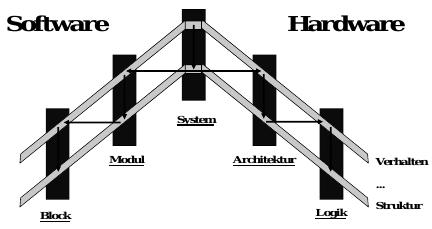
\includegraphics[scale=0.89]{pics/abstraktionsEbenen}
\end{figure}

\f{Abstraktionsebenen -- Software-Bereich}:
\begin{itemize}
 \item \ku{Modul}: die Modulebene gehört zum Softwarebereich. Die Modelle der Modulebene beschreiben komplexe Funktionen und ihre Interaktionen.
 \item \ku{Block}: die Blockebene gehört ebenfalls zum Softwarebereich. Die entsprechenden Modelle beschreiben Programme bis hin zu Instruktionen, die auf der 
 zugrundeliegenden Rechnerarchitektur elementare Operationen ausführen.
\end{itemize}

\f{Abstraktionsebenen -- Hardware-Bereich}:
\begin{itemize}
 \item \f{Architektur}: die Architekturebene gehört zum Hardwarebereich. Die Modelle dieser Ebene beschreiben kommunizierende Blöcke, die alle nebenläufig 
 komplexe Operationen ausführen.
 \item \f{Logik}: die Logikebene gehört ebenfalls zum Hardwarebereich. Die Modelle dieser Ebene beschreiben verbundene Gatter und Register, die Boolesche 
 Funktionen berechnen.
\end{itemize}

\f{Modell}:
\vspace*{3pt}

\noindent Unter einem Modell versteht man die formale Beschreibung eines Systems (oder Teilsystems). Wie genau ein Modell ein System beschreibt, hängt von der 
entsprechenden Abstraktionsebene ab. Man unterscheidet \idr zwischen 
\begin{itemize}
 \item \f{zustandsorientierten} (\zb auf endlichen Automaten basierende)
 \item \f{aktivitätsorientierten} (\zb auf Datenflussgraphen basierende)
 \item \f{strukturorientierten} (\zb auf Blockschaltbildern basierende)
 \item \f{datenorientierten} (\zb als Kollektion von Datenobjekten mit Relationen)
\end{itemize}
Modellen.
\vspace*{5pt}

\f{Aufgabe der (automatischen) Systemsynthese}:
\begin{itemize}
 \item Festlegung der Komponententypen, die in der Implementierung verwendet werden (Allokation), z.B. Mikroprozessor, ASIC, Speicherbausteine...
 \item Festlegung der Anzahl der jeweiligen Komponenten, Auswahl und Dimensionierung der Verbindungsstruktur (Allokation)
 \item Zuordnung der Variablen zu Speicherbausteinen, Operationen zu Funktionsbausteinen und Kommunikationen zu Bussen (Binding). Hierbei sind Realisierung in 
 Hardware und in Software gegeneinander abzuwägen (Hardware/Software-Partitionierung).
 \item Erstellung eines Ablaufplans: Wann wird welche Aufgabe durch seine Ressource ausgeführt?
 \item Schätzung von Systemeigenschaften, um eine vernünftige Exploration des Entwurfsraumes zu ermögli-chen. Gerade auf den obersten Entwurfsebenen werden 
 grundlegende Entwurfsentscheidungen getroffen, die die Leistungsfähigkeit und die Kosten des ganzen Systems bestimmen.
\end{itemize}

\f{Entwurfsablauf auf Systemebene}
\begin{figure}[!ht]
 \centering
 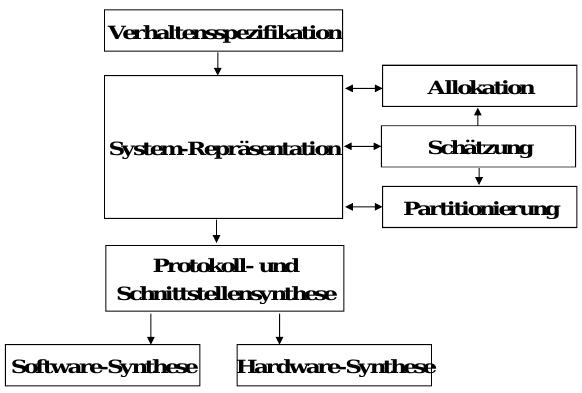
\includegraphics[scale=0.6]{pics/entwurfAufSystemebene}
\end{figure}

\f{Architektursynthese}

\noindent Aufgabe der Architektursynthese: eine strukturelle Sicht aus einer Verhaltensbeschreibung (\zb VHDL) zu generieren. $\Rightarrow$ Grad der Parallelität
\vspace*{5pt}

\ku{wesentlichste Aufgaben}:
\begin{itemize}
 \item Identifikation von Hardware-Elementen, die die spezifizierten Operationen ausführen können (Allokation)
 \item Ablaufplanung zur Bestimmung der Zeitpunkte, an denen die Operationen ausgeführt werden
 \item Binding, d.h. Zuordnung von 
 \begin{itemize}
  \item Variablen zu Speichern 
  \item Operationen zu funktionalen Einheiten
  \item Kommunikationskanäle zu Bussen
 \end{itemize}
\end{itemize}
\f{Modulsynthese}, \f{Logiksynthese}, \f{Blocksynthese}: werden in anderen Vorlesungen genauer behandelt

\section*{Chapter 1.2}
Formale Methoden zur Spezifikation von Systemen sind notwendig, um Realisierungen mit korrektem Verhalten synthetisieren zu können. Spezifizieren mit formalen 
Methoden ist nicht trivial... aber der einzige gehbare Weg!
\vspace*{3pt}

\f{Petri-Netze}
\vspace*{3pt}

\noindent \ku{Definition:}
Ein Petri-Netz ist ein 6-Tupel $G = (P,T,F,K,W,M_0)$ mit 
\begin{itemize}
 \item $P = \{p_1, \dots , p_m\}$ \dots die Menge der Plätze oder Stellen.
 \item $T = \{t_1, \dots , t_n\}$ \dots die Menge der Transitionen.
 \item $P \cap T = \varnothing$. Beide Mengen zusammen bilden die Menge der Knoten.
 \item $F \subseteq (P\times T)\cup(T\times P)$ \dots die Menge der Kanten. Auch Flussrelation genannt.
 \item $K:P \rightarrow N \cup \{\infty \}$, die jedem Platz eine Kapazität zuordnet
 \item $W:F \rightarrow N$, die jeder Kante ein Kantengewicht zuordnet.
 \item $M_0:P \rightarrow N_0$ mit $\forall p\in P:M_0(p)\leq K(p)$, die Anfangsmarkierung
\end{itemize}
Petri-Netze sind also gerichtete bipartite Graphen, denen man eine Interpretation im Sinne erreichbarer Markierungen gibt. Gängige Notation:
\begin{figure}[!ht]
 \centering
 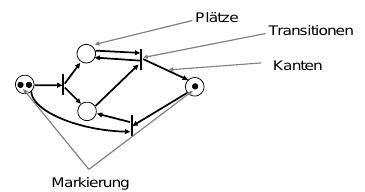
\includegraphics[scale=0.8]{pics/petrinetz}
\end{figure}

\f{Schreibweise}:
\begin{enumerate}
 \item $\forall t\in T:$ \textbullet$t = \{p;(p,t)\in F\}$: Vorbereich von t 
 \item $\forall p\in P:$ \textbullet$p = \{t;(t,p)\in F\}$: Vorbereich von p
 \item $\forall t\in T: t$\textbullet\ $ = \{p;(p,t)\in F\}$: Nachbereich von t 
 \item $\forall p\in P: p$\textbullet\ $ = \{t;(t,p)\in F\}$: Nachbereich von p
\end{enumerate}
\newpage

\f{Schaltbereitschaft von Transitionen}:
\begin{figure}[!ht]
 \centering
 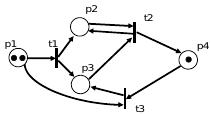
\includegraphics{pics/schaltbereitPetrinetz}
 \caption{Transitionen t1 und t3 sind schaltbereit}
\end{figure}

\noindent Eine Transition $t\in T$ eines Petri-Netzes schaltet von der Markierung $M$ auf $M'$: \[M[t>M'\]
\vspace*{5pt}

\f{Aktivierbare und lebendige Transitionen}
\vspace*{3pt}

\f{Definition}: \ku{Ist $M:P\rightarrow N_0$ eine Markierung eines Petri-Netzes, so heißt eine Markierung $M'$ des Petri-Netzes \f{erreichbar}, wenn}
\begin{itemize}
 \item $\exists t\in T:M[t>M'$
 \item $\exists t\in T:M''[t>M'$ und $M''$ ist von $M$ aus erreichbar
\end{itemize}
$[M>$ bezeichne die Menge der von M aus erreichbaren Markierungen.
\vspace*{6pt}

\noindent Eine Transition $t$ eines Petri-Netzes heißt bzgl. einer Markierung $M$ \f{tot}, wenn sie unter keiner von $M$ aus erreichbaren Markierung schaltbereit ist, 
d.h. $\forall M'\in [M>:\neg(M'[t>)$. Ansonsten heißt sie \f{aktivierbar}.
\vspace*{6pt}

\noindent Eine Transition $t$ eines Petri-Netzes heißt bzgl. einer Markierung $M$ \f{lebendig}, wenn sie bzgl. jeder von $M$ aus erreichbaren Markierung aktivierbar ist.
\vspace*{6pt}

\noindent Ein Petri-Netz heißt \f{deadlockfrei} oder \f{schwach lebendig}, wenn es zu jeder von $M_0$ aus erreichbaren Markierung $M'$ eine Transition $t\in T$ 
gibt, die schaltbereit ist.
\vspace*{6pt}

\noindent Ein Petri-Netz heißt \f{lebendig} oder \f{stark lebendig}, wenn jede seiner Transitionen bzgl. $M_0$ lebendig ist. 
\vspace*{6pt}

\noindent Sei G ein Petri-Netz und $B:P\rightarrow N_0 \cup \{\infty\}$ eine Abbildung, die jeder Stelle eine kritische Markenzahl zuordnet ($B(p)\leq K(p)$). 
Das Petri-Netz G heißt \f{B-sicher} oder \f{B-beschränkt}, wenn $ \forall M\in[M_0>\forall p\in P:M(p)\leq B(p)$.
\vspace*{6pt}

\noindent Das Petri-Netz heißt \f{sicher} oder \f{beschränkt}, wenn es eine natürliche Zahl $b$ gibt, für die G b-beschränkt ist. 
\vspace*{6pt}

\noindent Ein Petri-Netz ist genau dann beschränkt, wenn seine Erreichbarkeitsmenge $[M_0>$ endlich ist.
\vspace*{6pt}

\begin{figure}[!ht]
 \centering
 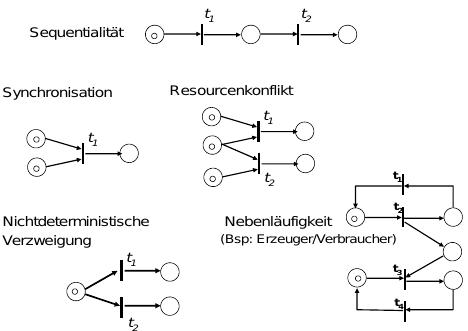
\includegraphics[scale=0.7]{pics/ausdruckPetrinetze}
 \caption{Ausdruckskraft von Petri-Netzen}
\end{figure}

\f{Überdeckung von Markierungen}:
\vspace*{4pt}

\noindent \ku{Annahme}: Die Kapazität eines Platzes ist unendlich. 
\vspace*{4pt}

\noindent Seien $M$ und $M'$ Markierungen. Dann ist $M+M'$ die Markierung, die man durch $M+M'(p) := M(p)+M'(p)$ erhält. Entsprechend sei ``-'' auf Markierungen 
definiert. 
\vspace*{4pt}

\noindent Eine Markierung $M$ \f{überdeckt} $M'(M\geq M')$ genau dann, wenn für alle Plätze $p$ gilt: $M(p)\geq M'(p)$
\vspace*{6pt}

\f{$\omega$-Erweiterungen}
\vspace*{4pt}

\noindent Eine $\omega$-erweiterte Markierung ist gegeben durch $M:P \rightarrow N_0 \cup (\omega)$
\vspace*{6pt}

\f{Überdeckungsgraph}
\vspace*{4pt}

\noindent Man kann nun zu jedem Petri-Netz wie folgt einen Überdeckungsgraphen von $M_0$ (ist ein Knoten des Graphen) aus konstruieren:
\begin{itemize}
 \item Knoten: $\omega$-erweiterte Markierungen $M:P\rightarrow N_0 \cup \{\omega \}$
 \item Kanten: Ist $M$ ein Knoten, dann ist für jede feuerbereite Transition $M[t>M'$ 
 
 \qquad \qquad  - $M'$ Nachfolgeknoten, falls kein Vorgänger $M''$ von $M$ existiert mit $M'\geq M''$
 
 \qquad \qquad  - $\Omega(M'',M')$ Nachfolgeknoten, falls $M''$ Vorgänger von $M$ mit $M'\geq M''$
\end{itemize}
\begin{itemize}
 \item Der Überdeckungsgraph ist stets endlich.
 \item Ein Petri-Netz ist beschränkt dann und nur dann, wenn bei der Konstruktion des Überdeckungsgraphen keine $\omega$-erweiterten Knoten entstehen
 \item Petri-Netze können den gleichen Überdeckungsgraphen haben und doch ungleiches Verhalten
 \item Bei beschränkten Petri-Netzen ist das Verhalten genau dann gleich, wenn die Überdeckungsgraphen isomorph sind
\end{itemize}

\begin{figure}[!ht]
 \centering
 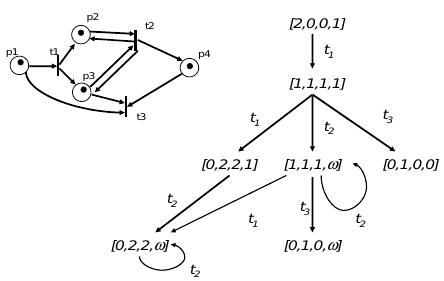
\includegraphics[scale=0.85]{pics/ueberdeckungsgraph}
 \caption{Beispiel für Überdeckungsgraph}
\end{figure}

\f{Zustandsorientierte Modelle}
\vspace*{6pt}

\noindent \f{Definition}: \\ \ku{Ein \f{endlicher} Automat ist gegeben durch ein 6-Tupel $M:=(I,O,S,R,\delta,\lambda)$}. 

\noindent Dabei sind $S,I,O$ endliche Mengen.

\qquad \qquad $S$ heißt \f{Zustandsmenge}, $R \subseteq S$ die Menge der \f{Startzustände} 

\qquad \qquad $I$ heißt \f{Eingabemenge} 

\qquad \qquad $O$ heißt \f{Ausgabemenge} 

\qquad \qquad $\delta:S\times I \rightarrow S$ heißt \f{Übergangsfunktion} 

\qquad \qquad $\lambda:S\times I\rightarrow O$ heißt \f{Ausgabefunktion}

\noindent sind $\lambda$, $\delta$ ``echte'' Relationen, nennt man den Automaten auch \f{nichtdeterministisch}. Sind $\delta$, $\lambda$ partiell, d.h. nicht 
für alle Paare $(s,x)$ definiert, nennt man den Automaten auch unvollständig. 

\noindent Es muss dann aber gelten, dass $\lambda(s,x)$ definiert $\Rightarrow$ $\delta(s,x)$ definiert.

\noindent Endliche Automaten können als Spezialfall interpretierter Petri-Netze aufgefasst werden. Ein nichtdeterministischer endlicher Automat ist ein 
Petri-Netz $G=(P,T,F,K,W,M_0)$ mit 
\begin{itemize}
 \item $\forall t\in T:|$\textbullet$t|=|t$\textbullet$|=1$
 \item $\exists p_0\in P:M_0(p_0) = 1$ und $\forall p\neq p_0:M_0(p) = 0$
 \item $K=W=1$
 \item jeder Transition ist ein Prädikat (Eingabeereignis) als zusätzliche Schaltbedingung und ein Ausgabeereignis als Aktion zugewiesen
\end{itemize}

\f{Statecharts}

\noindent Die Eingabesymbole endlicher Automaten sind in der Regel Sensorsignale oder Zustandssignale kooperierender Automaten. $\Rightarrow$ Notiere die Übergänge als 
Kanten mit Prädikaten (Ereignisse), die auf genau den Eingaben erfüllt sind, unter denen der Übergang stattfindet. 

\noindent Die Ausgabesymbole sind in der Regel Steuersignale für Aktoren. $\Rightarrow$ Notiere neben die Übergangsprädikate Aktionen.

\begin{figure}[!ht]
 \centering
 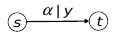
\includegraphics{pics/statechart}
 \caption{Unter allen Eingaben $x$ mit $\alpha(x)$ gehe mit Ausgabe $y$ nach $t$}
\end{figure}

\f{Statecharts -- Gruppierung}:

\noindent Gruppiere Zustände durch Einkreisen und erlaube Übergänge aus Zustandsgruppen. Ein Übergang aus einer Zustandsgruppe steht für Übergänge von jedem Zustand der 
Gruppe aus zu dem gegebenen Zielzustand. 

\begin{figure}[!ht]
 \centering
 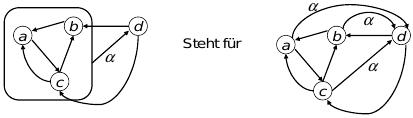
\includegraphics[scale=0.85]{pics/stateUebergang}
\end{figure}

\f{Statecharts -- Hierarchie}:

\noindent Gruppiere Zustände durch Einkreisen, benenne sie und markiere einen Startzustand. 
\begin{figure}[!ht]
 \centering
 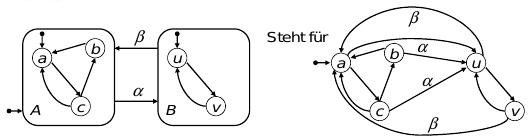
\includegraphics[scale=0.85]{pics/stateHierarchie}
\end{figure}

\f{Statecharts -- Nebenläufigkeit}:

\begin{figure}[!ht]
 \centering
 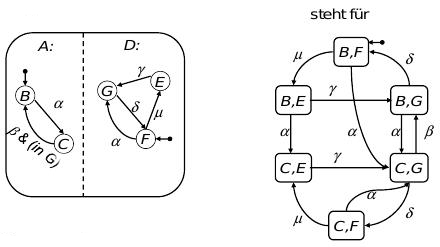
\includegraphics[scale=0.9]{pics/stateNeben}
\end{figure}

\newpage
\f{Datenflussgraphen - DFG}

\noindent DFGs sind gerichtete Graphen, die die durchzuführenden Berechnungen allein über die Verfügbarkeit der dazu notwendigen Daten definieren. Knoten 
entsprechen Operationen (Aktoren), Kanten entsprechen Datenabhängigkeiten. DFGs sind ein Sonderfall von Petri-Netzen: ersetze die Operationsknoten durch 
Transitionen und die Kanten durch Plätze:
\begin{figure}[!ht]
 \centering
 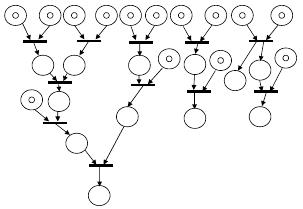
\includegraphics[scale=0.8]{pics/dfgPetri}
\end{figure}

\noindent Jeder Platz hat genau eine Nachfolge- und eine Vorgängertransition, denn jede Datenabhängigkeit hat genau einen Produzenten und genau einen Konsumenten
$\Rightarrow$ markierte Graphen 
\vspace*{6pt}

\f{Markierte Graphen}

\noindent \f{Definition}: \ku{Ein markierter Graph (MG) ist ein Petri-Netz $G=(P,T,F,K,W,M_0)$ mit folgenden Eigenschaften}:
\begin{itemize}
 \item $\forall p\in P: |$\textbullet$p| = |p$\textbullet$| = 1$
 \item $W=1$
 \item $\forall p\in P:K(p)=\infty$
\end{itemize}

\noindent Marken jeder Stelle $p$ werden in der Reihenfolge entnommen, in der sie dort entstehen (FIFO) $\Rightarrow$ keine Konflikte auf den Transitionen. Da in 
MG die Plätze stets genau einen Vorgänger und einen Nachfolger haben, kann man die Plätze auch als Knoten im Netz weglassen und direkt die Kanten zwischen 
Transitionen betrachten und markieren. 
\begin{figure}[!ht]
 \centering
 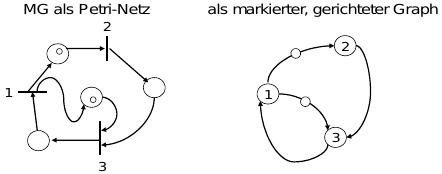
\includegraphics[scale=0.8]{pics/mgpetri}
\end{figure}

Ein Knoten kann feuern, wenn alle einlaufenden Kanten markiert sind. Er nimmt von jeder eingehenden Kante eine Marke und legt auf jede ausgehende Kante eine Marke. 

\noindent \f{Definition}: Ein markierter Graph ist ein gerichteter Graph $G=(V,E,M_0)$, wobei $M_0:E\rightarrow N_0$ die Anfangsmarkierungen der Kanten ist. 
\vspace*{6pt}

\f{Synchrone Datenflussgraphen}
\vspace*{3pt}

\noindent \f{Definition}: \ku{Ein synchroner Datenflussgraph (SDFG) ist ein Petri-Netz $G=(P,T,F,K,W,M_0)$ mit folgenden Eigenschaften}:
\begin{itemize}
 \item $\forall p\in P: |$\textbullet$p| = |p$\textbullet$| = 1$
 \item $\forall p\in P:K(p)=\infty$
\end{itemize}
\begin{figure}[!ht]
 \centering
 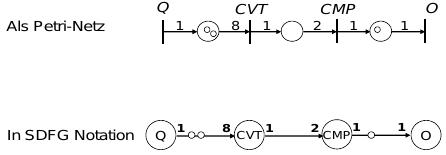
\includegraphics[scale=0.8]{pics/sdfg}
\end{figure}
\newpage
\noindent Marken jeder Stelle $p$ werden in der Reihenfolge entnommen, in der sie dort entstehen (FIFO). Im Unterschied zu markierten Graphen erhalten die Kanten echte 
Gewichte.

\f{Definition}: \ku{Ein SDFG $G$ ist ein 5-Tupel $G=(V,E,cons,prod,d)$ mit }
\begin{itemize}
 \item $V$ ist die Menge der Knoten -- Knoten stehen für Operationen
 \item $E\subseteq V\times V$ ist die Menge der Kanten -- aus Kanten können mehrere Daten liegen. Es gilt FIFO.
 \item $cons:E\rightarrow N$ gibt die Anzahl der beim Feuern des Zielknotens konsumierten Marken an -- sie stehen am Pfeilende
 \item $prod:E\rightarrow N$ gibt die Anzahl der beim Feuern des Quellknotens produzierten Marken an -- sie stehen am Pfeilanfang
 \item $d:E\rightarrow N_0$ gibt die Anfangsmarkierung der Kanten an, d.h. die Anzahl der anfangs auf jeder Kante verfügbaren Daten. 
\end{itemize}

\f{Topologiematrix des SDFG}

\noindent \f{Definition}: \ku{Sei $G=(V,E,cons,prod,d)$ ein SDFG. Die zu $G$ zugehörige Topologiematrix ist ein Matrix $C$ aus $Z^{|V|\times|E|}$, deren Zeilen 
den Knoten und deren Spalten den Kanten von $G$ entsprechen.} Verläuft die Kante $e_j$ vom Knoten $v_i$ zum Knoten $v_k$, so gilt 
\[C[i,j] := -prod(v_i,v_k)\]
\[C[k,j] := cons(v_i,v_k)\]
\[C[l,k] = 0 \text{ für } l\notin\{i,k\}\]
\begin{figure}[!ht]
 \centering
 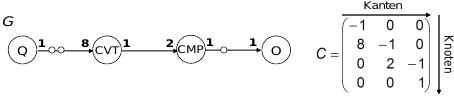
\includegraphics[scale=0.8]{pics/topologie}
\end{figure}

\noindent Ist $d_1$ die momentane Kantenmarkierung und feuert Knoten $v_i$ jeweils $y_i$-mal, so erhält man als resultierende Knotenmarkierung \[d_2 = d_1-C^T y\]
\vspace*{1pt}

\f{Definition}: \ku{Ein zusammenhängender SDFG $G$ mit Topologiematrix $C$ aus $Z^{|V|\times|E|}$ heißt konsistent, wenn die Startmarkierung in endlich vielen 
Schritten wieder angenommen werden kann, d.h. es ein periodisches Verhalten von $G$ gibt.}
\vspace*{4pt}

\noindent \f{Satz}: \ku{Ist $G$ zusammenhängend und konsistent, dann gilt $Rang(C) = |V|-1$}
\vspace*{3pt}

\f{Minimaler Repititionsvektor}
\vspace*{3pt}

\f{Definition}: \ku{Sei $G$ ein zusammenhängender, konsistenter SDFG. Dann heißt der kleinste positive Vektor $y \neq 0$ im Nullraum von $C^T$, d.h.}
\[y\in \{x\in N^{|V|}; C^Tx=0\} \sum_i y_i \text{ minimal}\] \ku{\f{minimaler Repititionsvektor} (von $G$).}
\begin{figure}[!ht]
 \centering
 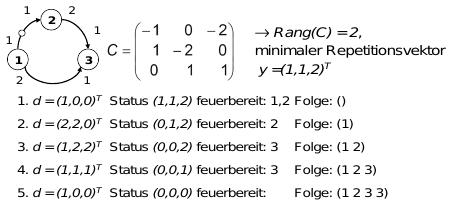
\includegraphics[scale=0.8]{pics/minRepVec}
\end{figure}

\newpage
\f{Verklemmung in SDFG}

\noindent Problem: mit der Existenz eines minimalen Repititionsvektors $y$ ist noch nicht sichergestellt, dass es zu diesem Vektor auch eine konkrete Folge 
schaltbereiter Knoten gibt, so dass jedes $v_i$ genau $y_i$-mal feuert. Das Netz könnte verklemmen. 
\begin{figure}[!ht]
 \centering
 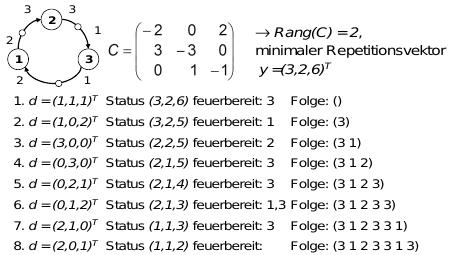
\includegraphics[scale=0.8]{pics/minRepVecVerkl}
 \caption{Beispiel für Verklemmung in einem SDFG}
\end{figure}

\f{Sequenzgraphen}

\noindent \f{Definition}: \ku{Ein Sequenzgraph ist ein azyklischer gerichteter Graph $G=(V,E)$ mit zwei ausgegzeichneten Knoten, einem Start- und einem 
Endknoten. Zusätzlich besitzt $G$ die folgenden Eigenschaften:}
\begin{itemize}
 \item die vom Start- und Endknoten verschiedenen Knoten lassen sich in die folgenden Klassen aufteilen:
 \begin{itemize}
  \item Operationsknoten 
  \item Hierarchieknoten
 \end{itemize}
 \item Hierarchieknoten sind Zeiger auf andere Sequenzgraphen. Man unterscheidet hierbei zwischen dem Modulaufruf (CALL), der Verzweigung (BR) und der Iteration 
 (LOOP) 
\end{itemize}

\section*{Chapter 1.3}
\begin{figure}[!ht]
 \centering
 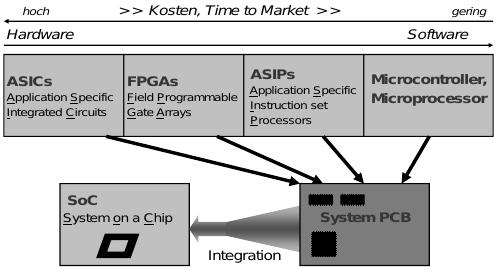
\includegraphics[scale=0.7]{pics/implementierung}
\end{figure}

\f{Allgemeines Synthesemodell}

\noindent \f{Gegeben ist:}
\begin{itemize}
 \item eine Menge von Aufgaben (Operationen, Tasks, \dots), die untereinander Datenabhängigkeiten besitzen können
 \item eine Menge von Ressourcen (ALUs, CPUs, Operatoren, \dots), auf denen jeweils gewisse Aufgaben ablaufen können 
\end{itemize}

\f{Gesucht ist:}
\begin{itemize}
 \item eine Festlegung der Anzahl von Ressourcen $\Leftarrow$ \f{Allokation}
 \item eine Festlegung des zeitlichen Ablaufs der Bearbeitung der Aufgaben unter Berücksichtigung der Datenabhängigkeiten $\Leftarrow$ \f{Ablaufplan (Schedule)}
 \item eine Zuordnung der Aufgaben zu den Ressourcen, so dass zu jeder Zeit jede Ressource höchstens eine Aufgabe bearbeitet $\Leftarrow$ \f{Bindung (Binding)}
\end{itemize}

Je nach Implementierungstechnik werden die Aufgaben unterschiedlich ausgeführt:
\begin{enumerate}
 \item \ku{Allokation}: dieses Problem wird in der Regel beim Entwurf gelöst und hat entscheidenden Einfluss auf die Kosten 
 \item \ku{Ablaufplan}: Ablaufpläne können beim Entwurf gelöst werden (statische Planung) oder zur Laufzeit (dynamische Planung), wobei dynamische Lösungen meist
 bei Softwareimplementierungen, statische eher bei Hardwareimplementierungen genutzt werden 
 \item \ku{Bindung}: Bindungen können ebenso als statische wie dynamische Aufgabe auftreten und von trivial (eine CPU) bis sehr schwierig (mehrere Ressourcen 
 gleichen Typs mit unterschiedlicher Leistung) rangieren
\end{enumerate}

\f{Definitionen}
\begin{itemize}
 \item \f{Sequenzgraph (Problemgraph, Taskgraph)} $G_S=(V,E)$. Sei ein gerichteter azyklischer Graph mit genau einem Start- und genau einem Endknoten. Im 
 folgenden bezeichnen wir mit $V_S\subseteq V$ die Knotenmenge $V$ ohne den Start- und Endknoten und mit $E_S \subseteq E$ die Kanten, die weder den Start- noch 
 den Endknoten als Randknoten besitzen. 
 \item bipartiter \f{Ressourcengraph} $G_R = (V_R, E_R)$ mit $V_R = V_S \cup V_T$ und $E_R \subseteq V_S\times V_T$. $V_T$ ist die Menge der Ressourcentypen 
 (\zb Prozessor, ALU, Addierer, \dots)
 \item \f{Kostenfunktion} $c:V_T\rightarrow N_0$, die die Kosten einer Instanz eines Ressourcentyps angibt 
 \item \f{Ausführungszeiten} $w:E_R\rightarrow N_0$, die jeder Kante $(v_s,v_t)\in E_R$ die Ausführungszeit der Aufgabe $v_S\in V_S$ auf einer Instanz des 
 Ressourcentyps $v_t \in V_T$ angibt
 \item ein \f{Syntheseproblem} $P$ ist gegeben durch ein Tupel $P = (G_S,G_R)$
\end{itemize}

\f{Definition -- Allokation}: \ku{Gegeben sei ein Syntheseproblem. Eine Allokation ist eine Funktion $\alpha:v_T\rightarrow N_0$, die jedem Ressourcentyp 
$v_t\in V_T$ eine Anzahl $\alpha(v_t)$ verfügbarer Instanz zuordnet.}
\vspace*{5pt}

\f{Definition -- Ablaufplan}: \ku{Gegeben sei ein Syntheseproblem. Ein Ablaufplan (Schedule) eines Sequenzgraphen $G_S=(V,E)$ ist eine Funktion 
$\uptau:V_S \rightarrow N_0$, die jedem Knoten $v_S \in V_S$ die Startzeit $\uptau(v_S)$ zuordnet und für jede Kante $(v_s,v_t)\in E_S$ die Bedingung}
\[\uptau(v_t) - \uptau(v_s)\geq w(v_s)\] 
\ku{erfüllt. Hierbei gibt $w(v_s)$ die Laufzeit der Aufgabe $v_s$ auf ihrer Ressource an.}

\f{Definition -- Latenz}: \ku{Die Latenz eines Ablaufplans $\uptau$ eines Sequenzgraphens $G_S = (V,E)$ ist definiert als}
\[L(\uptau) = \text{ späteste Beendungszeit $-$ früheste Startzeit } = max\{\uptau(v_i) + w(v_i); v_i \in V_S\} - min\{\uptau(v_j);v_j\in V_S\}\]

\f{Definition -- Bindung}: \ku{Eine Bindung eines Sequenzgraphens $G_S = (V,E)$ bzgl. eines Ressourcengraphen $G_R = (V_R,E_R)$ und einer Allokation 
$\alpha: V_T \rightarrow N_0$ ist ein Paar von Funktionen $\beta:V_S\rightarrow V_T$ und $\gamma:V_S \rightarrow N$ mit }
\begin{itemize}
 \item $\forall v_s \in V_S:(v_s,\beta(v_s)) \in E_R$
 \item $\forall v_s \in V_S:\gamma(v_s)\leq \alpha(\beta(v_s))$
\end{itemize}

\ku{d.h. die Bindung ordnet jeder Aufgabe eine verfügbare Instanz einer Ressource zu, die diese Aufgabe ausführen kann.}
Liegt ein Ablaufplan vor, so muss ferner gelten, dass zu jedem Zeitpunkt $t$ jeder Ressource nur eine Aufgabe zugeordnet ist.
\end{chapter}
